\documentclass{midl} % Include author names
%\documentclass[anon]{midl} % Anonymized submission
% \usepackage{biblatex}
% \addbibresource{midl-samplebibliography.bib}
% The following packages will be automatically loaded:
% jmlr, amsmath, amssymb, natbib, graphicx, url, algorithm2e
% ifoddpage, relsize and probably more
% make sure they are installed with your latex distribution

\usepackage{mwe} % to get dummy images

% Header for extended abstracts
\jmlrproceedings{MIDL}{Medical Imaging with Deep Learning}
\jmlrpages{}
\jmlryear{2020}

% to be uncommented for submissions under review
\jmlrworkshop{Short Paper -- MIDL 2020 submission}
\jmlrvolume{-- Under Review}
\editors{Under Review for MIDL 2020}

\title[Airway Labeling using Graph Neural Networks ]{Airway Labeling using Graph Neural Networks}

 % Use \Name{Author Name} to specify the name.
 % If the surname contains spaces, enclose the surname
 % in braces, e.g. \Name{John {Smith Jones}} similarly
 % if the name has a "von" part, e.g \Name{Jane {de Winter}}.
 % If the first letter in the forenames is a diacritic
 % enclose the diacritic in braces, e.g. \Name{{\'E}louise Smith}

 % Two authors with the same address
 % \midlauthor{\Name{Author Name1} \Email{abc@sample.edu}\and
 %  \Name{Author Name2} \Email{xyz@sample.edu}\\
 %  \addr Address}

 % Three or more authors with the same address:
 % \midlauthor{\Name{Author Name1} \Email{an1@sample.edu}\\
 %  \Name{Author Name2} \Email{an2@sample.edu}\\
 %  \Name{Author Name3} \Email{an3@sample.edu}\\
 %  \addr Address}


% Authors with different addresses:
% \midlauthor{\Name{Author Name1} \Email{abc@sample.edu}\\
% \addr Address 1
% \AND
% \Name{Author Name2} \Email{xyz@sample.edu}\\
% \addr Address 2
% }

%\footnotetext[1]{Contributed equally}

% More complicate cases, e.g. with dual affiliations and joint authorship
\midlauthor{\Name{Weiyi Xie %\midljointauthortext{Contributed equally}
% \nametag{$^{1,2}$}
} 
\Email{weiyi.xie@radboudumc.nl}\\
\addr Department of Radiology and\\
  Nuclear Medicine, Radboudumc\\
  Nijmegen, The Netherlands 1 \\
\AND
\Name{Colin Jacobs\midlotherjointauthor} \Email{colin.jacobs@radboudumc.nl}\\
\Name{Bram van Ginneken} \Email{bram.vanginneken@radboudumc.nl}\\ 
\addr Department of Radiology and\\
  Nuclear Medicine, Radboudumc\\
  Nijmegen, The Netherlands 1 
}

\begin{document}

\maketitle

\begin{abstract}
We propose a novel airway labeling approach in computed tomography (CT) based on graph attention networks. The proposed network formulates the airway labeling as the tree branch classification problem. We manually labeled six segmental branches according to their anatomical names. A convolutional neural network is  trained to classify each branch of the airway tree into one of these six labels or the others. Airway tree topology is implicitly embedded into a graph neural network to enrich convolutional features via pooling contextual information from neighboring branches. The final classification is performed using enriched features. The proposed method is evaluated on 100 subjects from COPDGene study. The results show that enriched features from the graph attention networks substantially improve the performance of airway labeling comparing to the raw convolution features, indicating that global knowledge on the airway tree helps the labeling of each anatomical branches.
\end{abstract}

\begin{keywords}
Graph Neural Networks, Airway Labeling, Computed Tomography.
\end{keywords}

\section{Introduction}
In chest Computed Tomography (CT), airway labeling is of importance for regional quantitative assessment of airway abnormalities. Airway labeling  is also vital in the virtual bronchoscope application to assist the navigation through airway tree and locate the target branch. Manual airway labeling is tedious and time-consuming, therefore an automation is necessary. In early studies, branch matching techniques \cite{kitaoka2002automated, tschirren2005matching, bulow2006point} were proposed to assign anatomical labels by matching the target tree against a pre-labeled airway tree using geometric and topological features such as orientations, inheritance relationship and topological distance at certain marker points.
Gaussian-based models\cite{van2008robust} were proposed to assign airway labels in a recursive schema where model parameters are found using branch features such as average radius, orientations and angles on manually labeled trees. A supervised hierarchical scheme \cite{feragen2012hierarchical} was later presented to label airway trees based on geodesic distance in a geodesic tree space. Many of these methods assumed a well-defined airway tree topology and relied on features that are sensitive to anatomical variation and imaging noise. 
In this paper, we use the same front-propagation technique as in \cite{van2008robust} to extract airway branches. Then we train a convolution neural network to extract features for each airway branch, and classify these branches to their anatomical names based on graph attention networks to capture the airway tree context. In this work, we focused on labeling segmental airways because given the segment branch labels and the airway tree structure, the remaining branch labels can be reconstructed trivially.

\section{Method}
\subsection{Data Selection}
We work with a set of 400 airway trees obtained from chest CT scans from the COPDGene study \cite{regan2011genetic}. The CT scans were inspiratory scans acquired at suspended full inspiration using 200 mAs and tube voltage of 120 KVP. The scans came from baseline subjects with normal, mild, moderate and severe COPD in terms of the GOLD standard \cite{rabe2007global}. 
Given an extracted airway tree and branch segmentations, analysts(trained medical students) manually labeled six segmental airway branches namely LB1, LB4, LB10 and RB1, RB4 and RB10 according to the Nomenclature from \cite{tschirren2005matching}. If auto-generated branch segments are inconsistent with the anatomical branching, analysts have to merge them or sketch the missing parts.

\subsection{Airway labeling Pipeline}
\begin{figure}[htbp]
 % Caption and label go in the first argument and the figure contents
 % go in the second argument
\floatconts
{fig:overview}
  {\caption{the baseline network(a) and the proposed network(b).}}
  {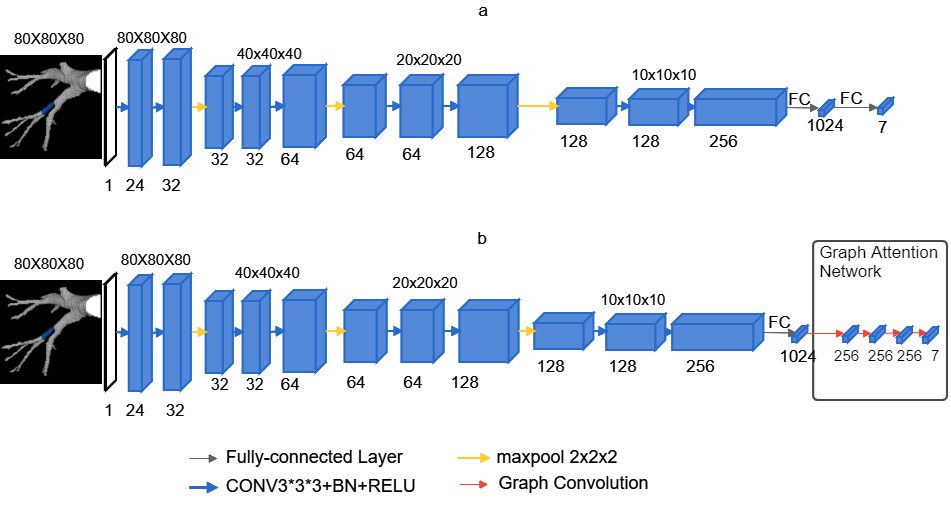
\includegraphics[width=0.95\linewidth]{resources/gnn_baseline.png}}
\end{figure}
Given a segmented airway tree, branches are extracted using wave front technique\cite{van2008robust}. A convolution neural network(CNN) is firstly trained to classify each branch into its anatomical name. The input to the CNN is a 3d patch cropped at the center of each branch at a resolution of 80x80x80 voxels. The CNN has three down-sampling blocks, and each consists of two convolutions with 3x3x3 filter of stride 1 and one max-pooling of 2x2x2 with stride 2. The down-sampled features are then feed into two consecutive convolutions before reshaped into a seven dimensional feature vector by two fully-connect layers. The softmax activation is used to provide 7-way class probabilities for a background class(other branches) and the six segmental airways.
The CNN is trained to classify anatomical labels until it converges. Then we freeze the layers before the last fully connect layer and use the 1024 dimensional feature vectors as the input to a graph attention neural network(GAN). The complete network architech is shown in Figure \ref{fig:overview}b.   
\subsubsection{Graph Attention Network}
A tree graph is constructed based on airway branch connectivity and the trachea is the root node. Each branch can be seen as a node in the tree graph and an edge is connected from the parent node to its children. In graph attention network, given $d$-dimensional feature representations of two connected nodes $h_{i}$, $h_{j} \in R^d$ , the edge weight(attention coefficient) $e_{ij}$ is computed as:
\begin{equation}\label{edge-weight}
    e_{ij} = \frac{exp(LeakyReLU(W_{r}^T[W_{g}h_{i}||W_{g}h_{j}]))}{\sum_{k \in N_{i}}exp(LeakyReLU(W_{r}^T[W_{g}h_{i}||W_{g}h_{j}]))}
\end{equation}
where $N_{i}$ represents the neighborhood of node $i$ in the graph.$W_{g}$ is a linear filter to project node presentations into a subspace. $||$ denodes the channel-wise concatenation. $W_{r}$ is a linear the transformation: $R^{2F} \rightarrow R$ to provide a scaler edge weight.
Once obtained, the normalized edge weights $e_{ij}$ are used to compute a linear combination of the features corresponding to them, to serve as the final output features for every node (after potentially applying a nonlinearity, $\sigma$):
\begin{equation}\label{edge-weight}
    h'_{i} = \sigma(\sum_{j \in N_{i}}e_{ij}W_{g}h_{j})
\end{equation}
To stabilize the learning process, we employ multi-head attention, similarly to \cite{vaswani2017attention}. 
In our experiments, the input dimension $d$ is 1024, and the number of head for each layer is set to 8. We use 4 graph attention layers, and each produces 256 dimensional feature vectors except the last layer which outputs a 7 dimensional vector for computing softmax classification probabilities.
Once all branches are classified, we perform a non-max suppression to leave only one predicted branch with the maximum estimated probability for each of the six target labels.  In the end, we output the center of the six predicted segmental branches as the results of the pipeline.  
\section{Results}
We compare our method(Figure \ref{fig:overview}b) with the baseline method which no graph attention network is used(Figure \ref{fig:overview}a). For assessing labeling performance, we compute overall accuracy(ACC) by checking whether the center of the predicted branch is inside the target branch. The results in Table \ref{tab:qresults} show that 

\begin{table}[htbp]
\floatconts
{tab:qresults}
  {\caption{Airway labeling performance: the proposed vs the baseline}}%
  {\begin{tabular}{ll}
  \toprule
  \bfseries Method & \bfseries ACC\\
  \midrule
  baseline & 0.679\\
  \midrule
  Proposed & 0.685\\
  \bottomrule
  \end{tabular}
  }
\end{table}

\midlacknowledgments{We thank Thirona for providing airway labeling annotations.}


\bibliography{midl-samplebibliography}


\end{document}
